% o \label{codigo} serve para podermos fazer referencias para algo numerado, 
% como capitulos, tabelas, figuras, etc. 
% Quando colocamos o comando \ref{codigo}. o compilador troca o \ref{codigo}
% pelo numero atribuido ao \label{}
% ex. \label{tabelaLegal}
%   A tabela \ref{tabelaLegal} mostra que...
% vai ser substituido por
%   A tabela 2 mostra que

\chapter{Teoria}\label{cap-teoria}

O desenvolvimento de um jogo educacional, que funcione como uma ferramenta de auxílio ao
aprendizado em sala de aula, deve envolver a consideração de diversos aspectos
pedagógicos, sociais e de \textit{game design}.

Em primeiro lugar, é necessário o estabelecimento de um vocabulário comum e bem
definido, delineando conceitos relevantes que possam ser empregados ao longo da 
formulação e desenvolvimento do projeto.

% ---
\section{Jogos Digitais}\label{sec-jogosdigitais}
% ---

\TODO{Será legal definir "jogo" antes? E "jogo digital educacional" depois?}

Para \cite{correia:2009:digital_games_spore}, jogos digitais são aqueles aonde exista
interação humano-computador, com o uso da tecnologia, e desenvolvidos para serem 
jogados em computadores, consoles ou outros dispositivos tecnológicos.

Tais jogos podem ser utilizados para auxiliar a assimilação de informações, permitindo
o aprendizado através de estratégias de ensino diferentes daquelas exploradas em sala
de aula, conforme demonstrado por \cite{fernandes:2012:digital_education}. Isto 
ocorre, em parte, por incentivar o aprendizado através da prática de atividades.

\cite{correia:2009:digital_games_spore} comprovam que a utilização de jogos 
na área de educação é importante não só pela motivação de se jogar um jogo, 
mas também pelo aprendizado através da exploração que ocorre. O 
desenvolvimento de jogos educacionais, porém, ainda é um desafio, devido 
à dificuldade de se juntar dois conceitos que parecem, a primeira vista,
ser discordantes: 'Educação' e 'Jogo'.

Para \cite{ramos:2013:jogos}, a inserção dos jogos digitais na educação 
contribui para o "desenvolvimento de aspectos cognitivos que são fundamentais 
para a aprendizagem", favorecendo o desenvolvimento de habilidades 
relevantes ao processo de aprendizagem. Adicionalmente, devido à 
grande quantidade de jogos digitais existentes, sua inclusão na sala 
de aula permite o acesso a um acervo muito grande e diversificado de 
novo conteúdo, com um custo baixo, que contribui com a "inclusão e 
alfabetização digital dos alunos". 

Os jogos que desafiam a lógica, considerado por \cite{ramos:2013:jogos} 
aqueles que "mobilizam o jogador a pensar, levantar hipóteses, 
experimentar, planejar, testar, realizar cálculos", contribuem uma
melhoria no desenvolvimento do raciocínio lógico, melhorando 
também habilidades de planejamento e atenção, além da percepção visual. 

% ---
\section{Mecânicas, dinâmicas e estética}\label{sec-mecanica-dinamica-estetica}
% ---

Segundo \cite{hunicke:2004}, um jogo, digital ou não, pode ser analisado através de
sua decomposição entre três componentes principais: mecânicas, dinâmicas e estética.

Mecânicas são entendidas como as regras efetivas do jogo, compondo as liberdades
concedidas e restrições impostas ao jogador, bem como seus objetivos, condições de
vitória e derrota. As mecânicas são a porção do jogo sobre a qual o desenvolvedor tem
controle direto, e influenciam a percepção das demais porções por parte do jogador.

Chamam-se de dinâmicas os comportamentos emergentes demonstrados por jogadores em 
função das mecânicas. Englobam desde comportamentos simples, como a reação de um
jogador a obstáculos do cenário, até sofisticadas estratégias a respeito de quando
cooperar ou competir em jogos multi-jogador.

Estéticas definem a experiência essencial que o jogador tem ao longo de uma sessão de
jogo. Diz respeito às respostas emocionais, ao envolvimento e à imersão do jogador no
mundo virtual criado pelo desenvolvedor, e é útil para categorizar o jogo quanto às
sensações que ele é capaz de invocar.

\TODO{Seria legal pegar um jogo 'conhecido' e explicar mecanicas, dinamicas e estética dele?}

% ---
\section{Realidade Virtual}\label{sec-realidadevirtual}
% ---

A Realidade Virtual é, de acordo com \cite{kirner:2007:RV_e_RA}, uma interface de
usuário avançada, que permite que o usuário veja, mova e interaja, em tempo real, 
com um ambiente tridimensional, através de dispositivos especiais. Em geral, a visão
tende a ser priorizada em interfaces de realidade virtual, mas a audição e o toque 
são também muito importantes para a experiência do usuário.

Para \cite{kirner:2011:evolucao_RV}, um mundo virtual visto através de uma tela é
considerado não-imersivo, enquanto a percepção deste mundo virtual através de salas 
com multiprojeção ou por meio de capacetes é considerado imersivo. Desta forma, a
realidade virtual:

\begin{alineas}
	\item considera a entrada e saída feita com equipamentos capazes de manipular 
	informação multisensorial em tempo real;
	\item prioriza interação em tempo real sobre a qualidade das informações;
	\item requer processamento gráfico, háptico e sonoro em alta escala;
	\item leva em consideração que ações ocorrem em um espaço tridimensional;
	\item considera que equipamentos especiais para a interação multisensorial sejam
	utilizados;
	\item entende que o usuário necessita de um período de adaptação para entender a
	representação virtual do mundo.
\end{alineas}

% ---
\section{Competências e Habilidades do Raciocínio Lógico}\label{sec-competenciashabilidades}
% ---

O Ministério da Educação (MEC) define um conjunto de parâmetros que devem estar
presentes no currículo de escolas em todo o Brasil. Estes são os Parâmetros
Curriculares Nacionais (PCN), e abordam várias diferentes áreas importantes. 

As competências e habilidades de raciocínio lógico consideradas para análise
consistem de um subconjunto dos PCN, em especial, daqueles relativos ao 
raciocínio lógico, e são apresentados no \autoref{quadro:PCN}, retirado de
\cite{Tabuti:2015:tabela_habilidades}.

\renewcommand{\arraystretch}{1.2}
\begin{quadro}[ht] \scriptsize
	\centering
	\caption[Competências e habilidades]{Competências e habilidades relacionadas ao raciocínio lógico.}
	\begin{tabular} {| >{\centering\arraybackslash} m{2cm} | >{\centering\arraybackslash} m{1.5cm} | m{7cm} |}
		\hline
		Competência & Habilidade & \multicolumn{1}{>{\centering\arraybackslash}p{7cm} |}{Descrição da habilidade} \\
		\hline
		\multirow{1}[12]{*}{Análise} & H1 & Habilidade em resolver um problema complexo dividindo-o em subproblemas mais simples, com soluções mais imediatas \\ \cline{2-3}
		& H2 & Habilidade da recomposição dos resultados gerados para a solução do problema mais complexo \\
		\hline
		\multirow{1}[40]{*}{Síntese} & H3 & Habilidade em juntar informações e dados de um problema que sejam de diferentes naturezas \\ \cline{2-3}
		& H4 & Habilidade em avaliar a deficiência dessas informações para determinar a solução\\ \cline{2-3}
		& H5 & Habilidade em descobrir a falta de outras informações necessárias para a resolução do problema  \\ \cline{2-3}
		& H6 & Habilidade em priorizar essas informações para o desenvolvimento até atingir a solução \\ \cline{2-3}
		& H7 & Habilidade em ordenar essas informações de forma a obter uma sequência de desenvolvimento até atingir a solução \\
		\hline
		\multirow{1}[28]{*}{Inferência} & H8 & Habilidade em descobrir padrões em um conjunto de informações \\ \cline{2-3}
		& H9 & Habilidade em aplicar novamente determinada informação de forma a agregar novas informações a estrutura de padrões existente \\ \cline{2-3}
		& H10 & Habilidade em aplicar novamente determinada informação de forma a agregar novas informações num conjunto que preserve a estrutura de padrões existente \\ 
		\hline
	\end{tabular}

	\legend{\fontedaimg{\cite{Tabuti:2015:tabela_habilidades}}}
	\label{quadro:PCN}
\end{quadro}

As três competências demonstradas na tabela são importantes para a resolução 
de problemas. O desenvolvimento da competência de análise permite a resolução
de problemas através da divisão em problemas menores que tenham soluções 
mais simples, assim como a recomposição dos resultados gerados para solucionar 
o problema mais complexo. O desenvolvimento da competência de síntese permite
combinar e ordenar diferentes informações obtidas, afim de chegar a uma solução
geral. O desenvolvimento da competência de inferência, por sua vez, permite
reutilizar informações, padrões e relações aprendidas em situações anteriores 
para solucionar problemas futuros.

% ---
\section{Público alvo}\label{sec-publico-alvo}
% ---

Uma vez estipulado que o foco do projeto seria na criação de um jogo que
auxiliasse no aprendizado e retenção de habilidades do raciocínio lógico,
e que este jogo seria criado para uma plataforma de realidade virtual,
foi necessário refinar cuidadosamente a escolha de público alvo de modo a
garantir que jogadores estivessem dentro de uma faixa etária para a qual 
experiências de realidade virtual fossem manejáveis, e para a qual a
aprendizagem de habilidades de raciocínio lógico fosse tão benéfica quanto
possível.

\subsection{Adaptabilidade à realidade virtual}

Uma consideração a ser feita foi a capacidade de crianças mais novas de
compreender e interagir com dispositivos de realidade virtual.

Enquanto muitos dos dispositivos encontrados no mercado atualmente sugerem
limites mínimos para a idade de seus usuários na faixa dos 12 e 13 anos de
idade \cite{seeto:2016:playstation-vr}, o pesquisador da Universidade da Califórnia Martin Banks afirma que
não existem comprovações de malefícios específicos a crianças advindos do
uso de equipamentos de realidade virtual, e que quaisquer efeitos adversos
que venham a incorrer sobre crianças novas fazendo uso destes equipamentos
seriam "os mesmos que aqueles sofridos por adultos" \cite{hill:2016:vr-safe}.

Banks publicou também em 2008 um artigo \cite{hoffman2008vergence} 
detalhando como \textit{displays}
tridimensionais e, por extensão, \textit{headsets} de realidade virtual,
não acarretariam nos malefícios causados por "\textit{near work}" - ou
seja, atividades de leitura ou foco visual em páginas e \textit{displays}
muito próximos ao rosto -, uma vez que este tipo de \textit{display} gera
pontos focais virtuais a uma distância confortável dos olhos, muito além
da distância do \textit{display} em si.

Apesar de não haver um limite rígido para a idade mínima para interação com
realidade virtual, como será necessário que as crianças consigam compreender
e interagir com ambientes tridimensionais, estipulou-se 8 anos de idade como
o mínimo necessário para fazer uso do jogo desenvolvido, pois a partir desta
idade pode-se considerar completo o domínio da criança sobre suas habilidades
motoras, segundo o \textit{Children’s Therapy \& Family Resource Centre} \cite{ctfrc:motor-skills}.

\subsection{Desenvolvimento do raciocínio lógico}
...

Com estas questões em mente, pretendeu-se então projetar um jogo voltado para
alunos do ensino fundamental, entre 8 a 12 anos, numa faixa etária suficiente
para interagir com as tecnologias empregadas e essencial para a formação de
suas capacidades de raciocínio lógico.

\TODO{Terminar}

% ---
\section{Tecnologia}\label{sec-tecnologia}
% ---

Para se desenvolver este projeto, foi necessário o estudo de algumas tecnologias, apresentadas a seguir. 
% ---
\subsection{Protocolo WebSocket}\label{subsec-teo-websocket}
% ---

O WebSocket é um protocolo de comunicação full-duplex que pode ser implementado
sobre uma conexão TCP, e foi padronizado em 2011 conforme descrito no RFC 6455
\cite{RFC:2011:websocket}. Ele foi desenvolvido para ser implementado em 
navegadores e servidores web, com o intuito de ampliar as possibilidades de
interação entre um navegador e um servidor. O protocolo permite que ambos os 
lados enviem mensagens ao outro a qualquer momento, sem a necessidade de um 
lado solicitar a mensagem. Mesmo tendo sido desenvolvido para uso em navegadores, 
o protocolo pode ser utilizado por qualquer aplicação de cliente e servidor.

Outro termo bastante relacionado ao WebSocket é o conceito de 
\textit{Push Notifications}, que são as mensagens enviadas de um servidor para 
um aplicativo executando em um celular para notificar o usuário de algum evento. 
O interessante é que o aplicativo não precisa ficar consultando o servidor 
(ex. \textit{polling}) para conseguir receber a mensagem, pois esta é enviada 
ao cliente quando o servidor quiser.

% ---
\subsection{Controlador Leap Motion}\label{subsec-teo-leap-motion}
% ---

O controlador \textit{Leap Motion}, da empresa de mesmo nome, começou a ser desenvolvido 
em 2008, contou com várias rodadas de investimento, e a primeira versão do 
\textit{Software Development Kit}(\textit{SDK}) foi lançada em maio de 2012. Dois anos depois, foi 
apresentada a segunda versão do \textit{SDK}, que melhorou bastante o rastreamento das 
mãos, e que é atualmente a versão mais utilizada. No início de 2016, a mais 
nova versão, chamada \textit{Orion}, foi lançada, desenvolvida especialmente para a 
realidade virtual, de acordo com \cite{leap:2016:changeset}

Para utilizar o controlador, são necessários 3 elementos diferentes: O hardware 
do controlador em si; um software rodando como um serviço em um computador; 
e um software 'cliente' que receberá os dados do serviço para utilizá-los, 
como pode ser visto na arquitetura do \textit{Leap Motion} \cite{leap:2016:architecture}

O controlador nada mais é do que um conjunto de duas câmeras e 3 LEDs, todos 
infravermelhos, de acordo com \cite{leap:2016:how-it-works}. Os LEDs projetam
luz infravermelha, que é refletida pelas mãos do usuário e captadas 
pelas câmeras. Estas imagens são enviadas ao serviço, 
que utiliza algoritmos de visão computacional para gerar modelos tridimensionais 
das mãos do usuário. A versão 2 do software aumentou muito a precisão do 
controlador por começar a trabalhar com um modelo esqueletal da mão, baseado 
na anatomia humana, ou seja, um modelo composto por 5 dedos, cada um contendo 
4 ossos. Este método insere restrições ao modelo, eliminando poses e movimentos 
que não seriam fisicamente possíveis.

O software cliente, então, pode receber os dados do serviço por duas interfaces:
Conversando diretamente com o serviço, utilizando uma biblioteca que acompanha o software, 
ou acessando o servidor \textit{WebSocket} que o serviço roda localmente.

A versão mais recente do \textit{SDK} ainda é nova, e tem focado na otimização dos 
algoritmos utilizados em várias áreas, tanto no processamento de imagens quanto 
outros algoritmos de 'suporte', como a detecção da adição ou remoção de um 
controlador. Visto a sua orientação para a realidade virtual, uma otimização 
importante foi em relação à mãos ocluídas, que sumiam em versões anteriores, 
conforme descrito em \cite{leap:2016:changeset}. É possível que comece a focar 
em coisas mais específicas para a realidade virtual em pouco tempo.

% ---
\subsection{Reconhecimento de Gestos}\label{subsubsec-teo-gestos}
% ---

\begin{figure}[h]
	\centering
	\caption{Modelo baseado na anatomia humana utilizado pelo controlador \textit{Leap Motion}}
	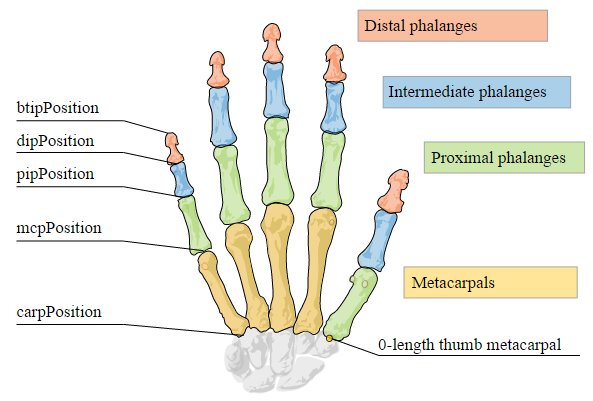
\includegraphics[width=0.7\textwidth]{leap-anatomical-hand}
	\legend{\fontedaimg{\cite{leap:2016:intro-skeletal}}}
	\label{fig:leap-anatomical-hand}
\end{figure}

Conforme mencionado na \autoref{subsec-teo-leap-motion}, a versão 
v2 em diante do controlador \textit{Leap Motion} utiliza um modelo 
da mão baseado na anatomia humana, conforme descrito 
em \cite{leap:2016:intro-skeletal}, e que pode ser visto 
na \autoref{fig:leap-anatomical-hand}. Isto significa que o 
rastreamento das mãos e dedos ficou mais preciso, pois a 
imagem capturada pelo controlador é processada e encaixada em 
um modelo anatomicamente correto. Desta forma, qualquer mão 
capturada terá 5 dedos, composto do número certo de ossos, e 
em posições e rotações anatomicamente possível. Isto também 
melhorou a oclusão de dedos, que antes sumiam do modelo da 
versão um(pois o modelo não teria necessariamente 5 dedos), 
agora podem ser estimados a partir do resto da mão.

A segunda versão do \textit{SDK} do \textit{Leap Motion} 
tinha, nativamente, o conceito de 'gestos', e o próprio 
\textit{SDK} disponibilizava alguns métodos para checar 
se alguns gestos básicos havia sido executado. Eram quatro 
o número de gestos reconhecidos: fazer um círculo com o 
dedo, deslizar o dedo, 'pressionar' um botão e tocar a 
tela, conforme descrito em \cite{leap:2016:gestures}. A 
versão \textit{Orion}, porém, no momento em que se 
iniciou o desenvolvimento deste trabalho, ainda não 
contava com a detecção automática de gestos, sendo 
necessário que o grupo desenvolvesse o código que o fizesse.

Dados os modelos das mãos, é possível detectar gestos através 
da posicão, rotação e velocidade da palma da mão, dos dedos, 
ou dos ossos individuais. Para a detecção de um dedo 
esticado, por exemplo, pode-se checar se o ângulo entre 
cada par de ossos adjacentes daquele dedo é \textit{pequeno} 
(aonde \textit{pequeno} deve ser definido com testes). 
Para se detectar uma palma virada para cima, pode-se 
verificar o vetor normal da palma (que nos é dada pelo 
\textit{SDK} do controlador) e ver se seu componente em 
y é positivo (tomando y como o eixo perpendicular ao 
plano do solo). Uma palma aberta apontando para cima, 
portando, pode ser detectada com o conjunto da detecção 
de um dedo esticado e da palma virada para cima.

É importante também notar que um mesmo gesto ou posicionamento
da mão pode ser descrita de várias formas. No caso do dedo esticado, 
por exemplo, poderia-se checar apenas o ângulo entre o primeiro e 
último ossos. Poderia, também, se calcular a distância entre estes
dois ossos. Dependendo do caso, as formas diferentes podem ser 
equivalentes, mas também podem apenas parecer iguais, mas quando
testados em ambientes diferentes, resultarão em saídas diferentes.
Por exemplo, uma mão menor poderia não ter o dedo considerado esticado
caso se utilizasse a distância entre os ossos.

Mais recentemente, porém, a empresa do \textit{Leap Motion} 
lançou módulos (chamados de \textit{utilities} no site) 
que permitem a detecção de gestos simples, não sendo 
mais necessário desenvolver código que o faça.

% ---
\subsection{Google Cardboard}\label{subsec-teo-google-cardboard}
% ---

O \textit{Google Cardboard} é um projeto da empresa Google criada em 2014 para 
fomentar o desenvolvimento de aplicações de realidade virtual. É composta por um 
\textit{headset} e de um software compatível. A ideia principal do projeto era
conseguir proporcionar a experiência de realidade virtual da forma mais barata 
o possível, conforme dito em \cite{cnet:2016:google-cardboard}. Para 
alcançar tal objetivo, o \textit{headset} é feito de papelão, 
de tal forma que o único subcomponente mais caro seja as lentes. Adicionalmente, 
um celular é utilizado tanto como poder de processamento do \textit{headset} 
quanto como a tela deste. Visto que uma grande parcela da população ja tem um 
\textit{smartphone}, estas partes do \textit{Cardboard} vêm de graça.

Quanto ao software compatível, é necessário que este divida a sua saída de 
vídeo (que será mostrado na tela do celular) em metades, uma para cada olho. 
Visto que cada imagem emula a visão de um olho, é necessário que as imagens 
venham de pontos de origem separados por uma distância equivalente àquela entre 
as duas pupilas, valor que varia entre 58 mm e 70 mm, de acordo com
\cite{dodgson:2004:svariation}. Adicionalmente, devido à distorção causada 
pelas lentes, é necessário que o software aplique a distorção inversa na imagem, 
de forma que a imagem após passar pela lente fique correta. É também necessário 
ler sensores encontrados no dispositivo móvel, como acelerômetros e giroscópios, 
e disponibilizar estes dados para que se possa implementar o movimento do 
usuário dentro do jogo ou aplicativo.

O \textit{SDK} do \textit{Google Cardboard}, distribuído pela própria Google e disponível online 
em \cite{google:2016:cardboardSDK}, já faz todas estas transformações necessárias 
na imagem, além de enviar os dados de movimento, ja processados, de volta ao
software que esteja utilizando o \textit{SDK}.
